\documentclass[14pt]{extarticle}
\usepackage{amsmath}
\usepackage{amssymb}
\usepackage{tikz}
%\usetikzlibrary{calc}
\usetikzlibrary{trees}
\usepackage{hyperref}
\usepackage{graphicx}
\graphicspath{ {../../chap09/} }
\usepackage[top=0.75in, bottom=0.75in, left=0.75in, right=0.75in]{geometry}
\newcommand*{\Scale}[2][4]{\scalebox{#1}{\ensuremath{#2}}}%
\usepackage[shortlabels]{enumitem}
\usepackage[most]{tcolorbox}
\definecolor{bg}{RGB}{255,249,227}
% \usepackage{showframe}
\usepackage{caption}
\usepackage{fdsymbol}


\title{\vspace{-5ex}HANDOUT Math 208 Week 08}
\date{\vspace{-10ex}}
\usepackage{multicol}
\setlength{\columnsep}{.5cm}

\begin{document}
\maketitle		

\section{Section 9.1}
\begin{center}
	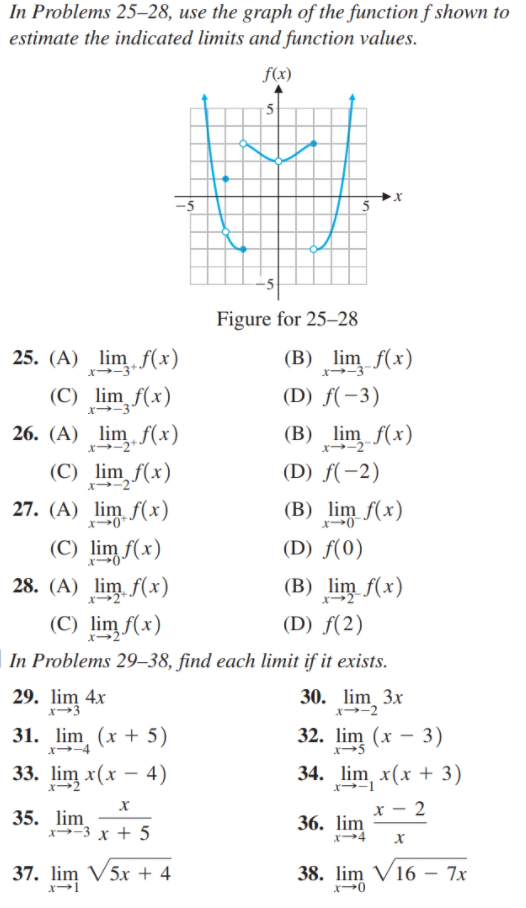
\includegraphics[width=0.7\linewidth]{9-1-7} \\
	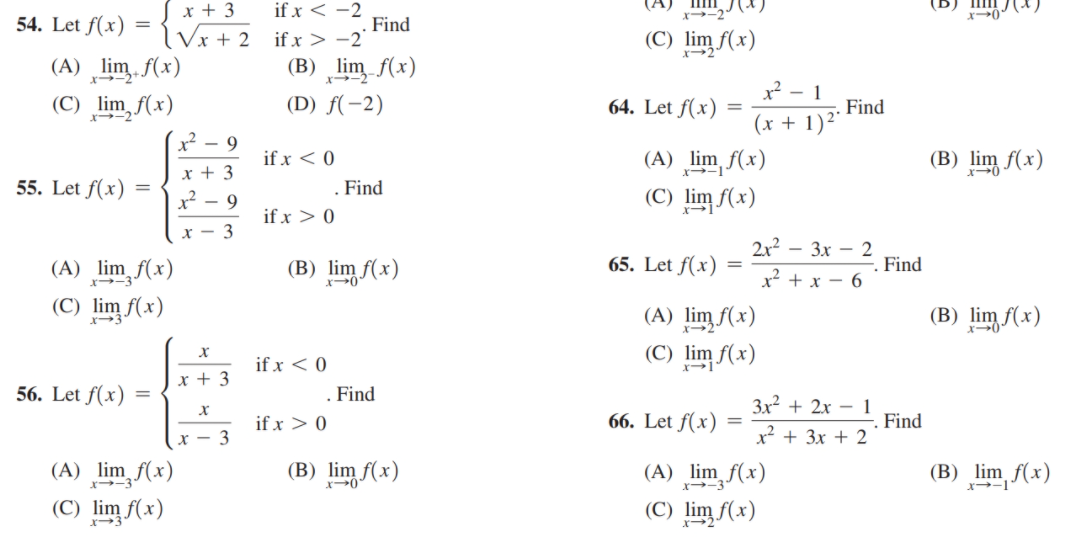
\includegraphics[width=1.0\linewidth]{9-1-8} \\
\end{center}

\subsection*{Section 9.2: Infinite Limits}
\begin{center}
	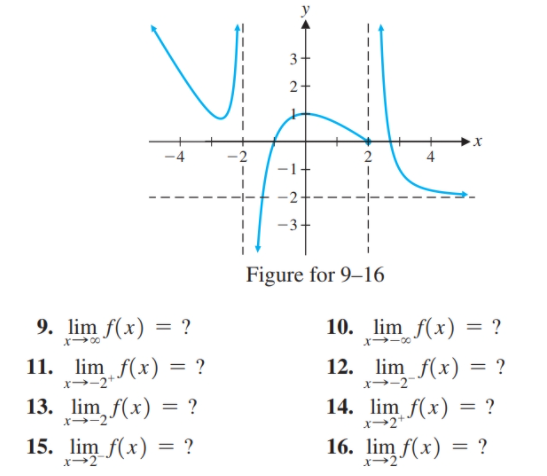
\includegraphics[width=0.8\linewidth]{9-2-8} \\
	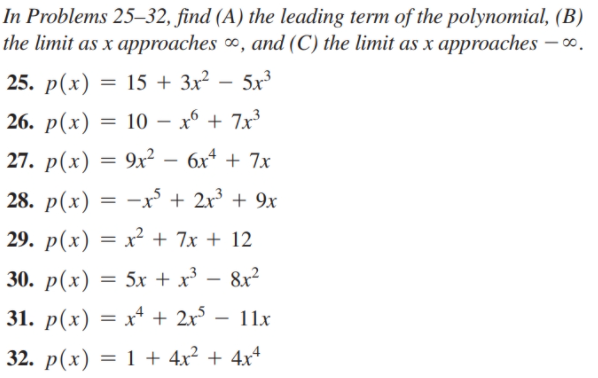
\includegraphics[width=0.8\linewidth]{9-2-9} \\
	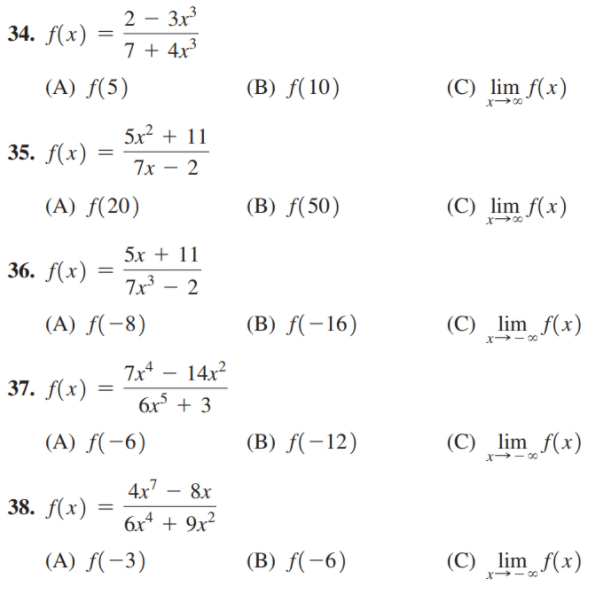
\includegraphics[width=0.74\linewidth]{9-2-10} \\
\end{center}

\section{Section 9.4}
\begin{center}
	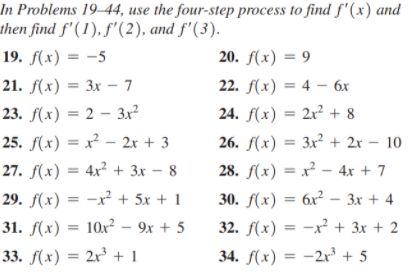
\includegraphics[width=0.7\linewidth]{9-4-20b}
\end{center}
Find the equation of the tangent line at $x=2$ for numbers 22 and 26.




\noindent\rule{\textwidth}{1pt}
{\footnotesize Copyright (C) 2021 Garold Dalton --- Released under GNU General Public License v3.0}


\cleardoublepage


\end{document}
